% nie rusza�
\RequirePackage{ifpdf}
\newif\ifelektroniczna
\newif\ifjednostronna
\newif\ifprojektInzynierski

%%%%%%%%%%%%%%%%%%%%%%%%%%%%%%%%%%%%%%%%%%%%%%%%%%%%%%%%%%%%%%%%%%%%%%%%%%%%
% USTAWIENIA GLOBALNE I domy�lna �cie�ka do plik�w z obrazkami, kodowanie itp. 
% okre�lone s� w drugiej sekcji ustawie�

% czy projekt czy praca magisterska
\projektInzynierskitrue % projekt
%\projektInzynierskifalse % praca magisterska

% czy wersja elektroniczna (pdf z kolorowymi linkami) czy nie (np. do druku)
\elektronicznatrue
%\elektronicznafalse

% czy jednostronna (recenzent), czy dwustronna (do akt);
% UWAGA: to nie jest dyrektywa dla drukarki; nie zmienia sposobu wydruku, 
% tylko to, w jaki spos�b rozpoczynane s� rozdzia�y, ustawiane marginesy
% itp.

%\jednostronnafalse
\jednostronnatrue

%%%%%%%%%%%%%%%%%%%%%%%%%%%%%%%%%%%%%%%%%%%%%%%%%%%%%%%%%%%%%%%%%%%%%%%%%%%%


% nie rusza�
\ifjednostronna
    \def\strony{oneside,openany}
\else
    \def\strony{twoside,openright}
\fi

\ifpdf
    % uwaga, ustawiaj�c co� innego ni� 12 sprawd� uk�ad strony tytu�owej (marginesy)
    \documentclass[pdftex,12pt,a4paper,\strony,colorlinks,nocenter,noupper,crosshair]{thesis}
    \usepackage[pdftex]{graphicx}
    \pdfcompresslevel=1
\else    
    \documentclass[12pt,a4paper,\strony,nocenter,noupper,crosshair]{thesis}
    \usepackage{graphicx}
\fi

% nie rusza�
\usepackage{url}
\usepackage{stronatytulowa}

%%%%%%%%%%%%%%%%%%%%%%%%%%%%%%%%%%%%%%%%%%%%%%%%%%%%%%%%%%%%%%%%%%%%%%%%%%%%
% USTAWIENIA GLOBALNE - cz�� 2
%

% kodowanie dokumentu
%\usepackage[utf8]{inputenc}   % linuks/windows/mac; pozwala na �atwe mieszanie znak�w z r�nych j�zyk�w
\usepackage[cp1250]{inputenc} % windows

% dane 
\ifprojektInzynierski
    \def\rodzaj{Projekt z Bioniki}
\else
    \def\rodzaj{Praca dyplomowa magisterska}
\fi
%\def\rodzaj{Praca przej�ciowa}

% stan na 2011-2012
\ifprojektInzynierski
    \def\wydzial{In�ynierii Biomedycznej}
\else
    \def\wydzial{In�ynierii Biomedycznej}
\fi

\def\tytul{Wykorzystanie sieci neuronowych\\ do wyznaczania optymalnej ilo�ci snu \\dla konkretnego cz�owieka} % Prosz� u�y� i ma�ych, i du�ych liter!
\def\autor{Autor: Dawid Bara�ski} %Jan Kowalski a NIE JAN KOWALSKI

% tytu� i autor dla pdfa - najcz�ciej jw, ale bez podzia�u na liniie i BEZ POLSKICH LITER
\def\tytulpdf{dawid_baranski_bionika_projekt}
\def\autorpdf{Dawid Baranski}

% promotor
\def\promotor{Kieruj�cy prac�: dr Barbara Mika} % prof. nzw. dr hab. in�. dr n.med doc. Jan Kowalski

% z konsultantem/bez konsultanta
%\def\konsultant{Konsultant: Konsultant} prof. nzw. dr hab. in�. dr n.med doc. Jan Nowak
\def\konsultant{}

\def\data{Zabrze, maj, 2018} % uwaga na wielko�� liter: grudzie� 2012/czerwiec 2012/..

% do pdfa
\def\slowakluczowe{SLOWA,KLUCZOWE}

% �cie�ka do obrazk�w
\graphicspath{{./rysunki/}}

% ustawienia dla pdfa
\ifpdf
\ifelektroniczna
     \usepackage[pdfusetitle=true,
	  pdfsubject={\tytulpdf},
	        pdfkeywords={\slowakluczowe}, 
		pdfcreator={\autorpdf},
		pdfstartview=FitV,
		linkcolor=blue,
		citecolor=red,
		]{hyperref}
\fi                 
\fi


\usepackage{layout}% poka� marginesy

% Nazwa za��cznik�w 
\def\appendixname{Za��cznik}
%%%%%%%%%%%%%%%%%%%%%%%%%%%%%%%%%%%%%%%%%%%%%%%%%%%%%%%%%%%%%%%%%%%%%%%%%%%%

% nie rusza� (cho� chwilowo niepotrzebne)
%	\author{\autor}
%	\title{\tytul}
%	\date{\data}
%

% === PAKIETY ===
\usepackage{url}

% �adne czcionki dla PDF + ustawienia spolszczaj�ce
\usepackage{t1enc,amsmath}
\usepackage[OT4,plmath]{polski}

% potrzebne dla strony tytu�owej:
\usepackage{helvet} 

% pierwszy paragraf w rozdziale/sekcji powinien by� wci�ty
\usepackage{indentfirst}

% marginesy
%\usepackage{anysize}
%\marginsize{3cm}{2.5cm}{2.5cm}{2.5cm}%LPGD
%\setlength{\textheight}{24cm}
% za spraw� thesis
%\textwidth 150mm
%\textheight 225mm

% czcionki matematyczne
\usepackage{amsfonts}

% rysunki z�o�one z wielu [pod]rysunk�w
\usepackage{subfig}
\captionsetup[subfigure]{justification=centerfirst}

% mo�liwo�� sklejania wierszy tabeli
\usepackage{multirow}

% mo�liwo�� wklejania adres�w - jest ju� w��czony wy�ej
%\usepackage{url}

% ulepszona obs�uga cytowa�
\usepackage{cite}

% listingi
\usepackage{listings}
% domy�lne ustawienia (niestety utf8 nie jest akceptowany)
%\lstset{language={Matlab},inputencoding=cp1250}}
%\lstset{language={Matlab},inputencoding=latin2}}
\lstset{language={Java},inputencoding=latin2} % powinno pasowa� te� do C#

% \addcontentsline nie dzia�a za dobrze w po��czeniu z hyperref, ale to nie dzia�a z klas� thesis
%\usepackage[nottoc]{tocbibind}

% strona po cleardoublepage powinna by� pusta, nie z nag��wkami
\usepackage{cleardpempty}

% == opcjonalne

% wymu� po�o�enie grafiki (itp.) przez [H]
\usepackage{float} 

% znak promila i inne znaki specjalne
%\usepackage{textcomp}

% je�li trzeba obr�ci� stron� (wstawi� co� w orientacji poziomej), u�yj tych pakiet�w
%\ifpdf\usepackage{pdflscape}\else\usepackage{lscape}\fi

% je�li potrzebujesz d�ugich tabeli (wiele stron)
%\usepackage{longtable}

% === POLECENIA DODATKOWE ===

% wektor w tek�cie
\def\vec#1{\ensuremath{\mathbf{#1}}}

% anglicyzmy i �acinizmy
\def\ang#1{ang.~\emph{#1}}
\def\lat#1{�ac.~\emph{#1}}

% proste e (jako podstawa logarytmu naturalnego) we wzorach i w tek�cie:
\def\e{\ensuremath{\textrm{\normalfont{}e}}}

% znak stopnia [jak w "5 stopni"]
\def\stopien{\ensuremath{^{\circ}}\protect\space}

% notatki na marginesie
\def\fixme#1{\marginpar{\tiny{}#1}}
%\def\fixme#1{} % gdy nie chcemy ich drukowa�, wystarczy zast�pi� powy�sze tym

%ODNOSNIKI 
% �eby wykorzysta� przypis dwukrotnie; druga wersja gorzej dzia�a�a w po��czeniu 
% z hyperref; czyli \footnote{blablabla \label{przypisX}} + \footnotereuse{przypisX}
%\newcommand{\footnreuse}[1]{\raisebox{1ex}{\scriptsize{}\protect\ref{#1}}}

% == �RODOWISKA DLA TWIERDZE�, LEMAT�W itp. ===
\newtheorem{twierdzenie}{Twierdzenie}[chapter]
\newtheorem{wlasnosc}{W�asno��}[chapter]
\newtheorem{lemat}{Lemat}[chapter]
\newenvironment{dowod}{\parindent=0pt{\bf Dow�d. }}{\begin{flushright}$\square$\end{flushright}}

% === RACZEJ NIE RUSZA� ===

%\usepackage{makeidx}
%\makeindex
%\usepackage{threeparttable}
%\usepackage[small,center]{caption2}

\def\captionlabeldelim{.}

%\usepackage{geometry}
%GATHER{thesis.bib}
%\usepackage[twoside]{geometry}
%\geometry{ lmargin=3.5cm, rmargin=2.5cm, tmargin=3cm, bmargin=3cm,
%headheight=1cm, headsep=0.5cm, footskip=0pt }

\linespread{1}
\chapterfont{\Huge\bfseries}
\sectionfont{\bfseries\Large}
\subsectionfont{\bfseries\large}
\institutionfont{\bfseries}%\mdseries}
\def\captionlabelfont{\bfseries}

\renewcommand{\figureshortname}{Rys.}
\renewcommand{\tableshortname}{Tab.}

\renewcommand\floatpagefraction{.9}
\renewcommand\topfraction{.9}
\renewcommand\bottomfraction{.9}
\renewcommand\textfraction{.1}
\setcounter{totalnumber}{50}
\setcounter{topnumber}{50}
\setcounter{bottomnumber}{50}

\newcommand{\topcaption}{%                  % robi podpis nad tabelk� z odst�pem po podpisie
   \setlength{\abovecaptionskip}{0pt}%
   \setlength{\belowcaptionskip}{10pt}%
   \caption}



% marginesy
\usepackage{anysize}
\marginsize{3cm}{2.5cm}{2.5cm}{2.5cm}%LPGD
%\setlength{\textheight}{24cm}
% za spraw� thesis
%\textwidth 150mm
%\textheight 225mm

\begin{document}
%
\bibliographystyle{acm}
%

%
\stronatytulowa
\titlepage
%-\cleardoublepage % je�li dwustronnie, to druga strona powinna by� pusta
\frontmatter 
%\maketitle

%\tocbibname

\tableofcontents \listoffigures \listoftables
%\listofacros
%\input{abbrev_body}
%\newpage
%\input{spis_oznaczen}

\mainmatter % <--- to + frontmatter powy�ej odpowiada za fakt, �e numerowanie jest od 1!
\chapter{Wst�p}
�Sen to stan obni�enia wra�liwo�ci na bod�ce, cz�ciowej bezw�adno�ci i zwolnienia funkcji, po��czony ze zniesieniem �wiadomo�ci, wyst�puj�cy u cz�owieka i zwierz�t wy�szych w rytmie dobowym, na przemian z czuwaniem.� \cite{MedycynaSnu}

% !TeX root = Praca.tex
\section{Cel projektu}
Celem projektu by�o stworzenie narz�dzia, s�u��cego do wyznaczania optymalnej ilo�� snu dla konkretnego cz�owieka. Danymi by�y odczyty o ilo�ci i jako�ci snu z poprzednich dni.

\section{Optymalna ilo�� snu}
Z bada� przeprowadzonych przez Centers for Disease Control and Prevention (CDC)\cite{statistics} wynika, �e zdrowy sen powinien trwa� przynajmniej 7 godzin. W�r�d m�odzie�y wi�cej, bo mi�dzy 8 a 10 godzin. 

Inne badania wykaza�y, �e minimalna ilo�� snu, potrzebnego do prawid�owego funkcjonowania organizmu to 6 godzin. Przy czym sen poni�ej 4,5 godziny mo�na uzna� za niebezpieczny dla kom�rek nerwowych m�zgu.

Nie jest jednak mo�liwe, wyznaczenie jednej optymalnej ilo�ci snu dla wszystkich ludzi. Du�y wp�yw na regeneracj� organizmu ma nie tylko ilo��, ale tak�e jako�� snu. 

\section{Zaburzenia powodowane brakiem snu}
D�ugoterminowe badanie Gallup z 2013 roku wykaza�o, �e w�r�d Amerykan�w 40\% spo�ecze�stwa �pi poni�ej 6 godzin. Nale�y zauwa�y�, �e w�r�d ostatnich 30 lat, ilo�� snu ustali�a si� na r�wnym poziomie. 14\% Amerykan�w sypia mniej ni� 5 godzin na dob�, jednak w latach 40 by�o to zaledwie 3\%. Problem dotyczy te� nastolatk�w 2/3 z nich sypia mniej ni� 8 godzin. Dostarczanie organizmowi zbyt ma�ej ilo�ci snu mo�e wp�ywa� na ryzyko zachorowa� na wiele chor�b. 

W tabeli (Tab.~\ref{Zaburzenia_snu}) przedstawiono wyniki bada� dotycz�cych wyst�powania 10 chronicznych chor�b, w por�wnaniu do ilo�ci snu. Jako pr�g przyj�to 7 godzin snu. Przebadano 2000 os�b ze standardowej populacji.  Wykazano jednoznacznie, �e d�u�szy sen pozytywnie wp�ywa na nasze zdrowie. Mo�e chroni� przed takimi chorobami jak nowotw�r czy cukrzyca. 

\begin{table}[]
\centering
\caption{Zaburzenia powodowane kr�tkim snem}
\label{Zaburzenia_snu} \cite{statistics}
\def\arraystretch{1.5}%  1 is the default, change whatever you need
\begin{tabular}{|l|l|l|l|l|}
\hline
                               & \multicolumn{2}{l|}{\textbf{Kr�tki sen (\textless{}7 godzin)}} & \multicolumn{2}{l|}{\textbf{Sen (\textgreater{}7 godzin)}} \\ \hline
\textbf{Przewlek�e schorzenie} & \textbf{\%}                  & \textbf{95\% P}                 & \textbf{\%}                       & \textbf{95\% P}                      \\ \hline
Atak serca                     & 4.8                          & (4.6�5.0)                       & 3.4                               & (3.3�3.5)                            \\ \hline
Choroba wie�cowa serca         & 4.7                          & (4.5�4.9)                       & 3.4                               & (3.3�3.5)                            \\ \hline
Udar m�zgu                     & 3.6                          & (3.4�3.8)                       & 2.4                               & (2.3�2.5)                            \\ \hline
Astma                          & 16.5                         & (16.1�16.9)                     & 11.8                              & (11.5�12.0)                          \\ \hline
Obturacyjny bezdech senny      & 8.6                          & (8.3�8.9)                       & 4.7                               & (4.6�4.8)                            \\ \hline
Nowotw�r                       & 10.2                         & (10.0�10.5)                     & 9.8                               & (9.7�10.0)                           \\ \hline
Artretyzm                      & 28.8                         & (28.4�29.2)                     & 20.5                              & (20.2�20.7)                          \\ \hline
Depresja                       & 22.9                         & (22.5�23.3)                     & 14.6                              & (14.3�14.8)                          \\ \hline
Przewlek�a choroba nerek       & 3.3                          & (3.1�3.5)                       & 2.2                               & (2.1�2.3)                            \\ \hline
Cukrzyca                       & 11.1                         & (10.8�11.4)                     & 8.6                               & (8.4�8.8)                            \\ \hline
\end{tabular}
\end{table}



\section{Jako�� snu}
Poprzez jako�� snu definiuje si� mo�liwo�� regeneracji organizmu podczas snu w jednostce czasu. Istotny wp�yw ma �rodowisko w jakim �yjemy, uwarunkowania genetyczne oraz sytuacje wynikaj�ce z konkretnego dnia. Za wprowadzenie w stan snu i jego jako�� odpowiada hormon melatonina.

"Melatonina jest wytwarzana w nocy, niezale�nie od tego o jakiej porze �pimy. Produkowana wy��cznie w ciemno�ci. Prawdopodobnie wzrasta po przyj�ciu pokarmu." \cite{melatonina} Jest najwa�niejszym czynnikiem wp�ywaj�cym na jako�� snu. W�r�d czynnik�w �rodowiskowych, negatywnie oddzia�uj�cych na sen, mo�na wymieni� stresuj�cy tryb �ycia, zmienn� por� snu, czy brak aktywno�ci fizycznej. 

Wed�ug National Sleep Foundation, g��wnymi kluczami determinuj�cymi jako�� snu s�:
\begin{itemize}
\item czas snu w odniesieniu do ca�kowitego czasu w ��ku (przynajmniej 85\%)
\item zasypianie w mniej ni� 30 minut
\item maksymalnie jedno przebudzenie w ci�gu nocy
\item przebudzenie trwaj�ce nie d�u�ej ni� 20 minut
\end{itemize}
Szczeg�ow� charakterystyk� snu mo�na przeprowadzi�, stosuj�c badanie elektroencefalograficzne (EEG). Wynikiem jest wykres bioelektrycznej czynno�ci m�zgu. Analizuj�c prac� m�zgu, mo�na wyr�ni� fazy. 

\section{Charakterystyka snu}
\subsection{Fazy snu}
Sen dzieli si� na dwie fazy:

- faza NREM (z ang. non-rapid eye movement) to sen wolnofalowy -  m�zg wy��cza wi�kszo�� funkcji, oddech staje si� regularny, spada ci�nienie t�tnicze, napi�cie mi�ni zanika, a co najwa�niejsze do krwi uwalniany jest hormon wzrostu.

- faza REM (z ang. rapid eye movement) to sen paradoksalny  � sen o szybkich ruchach ga�ek ocznych. Mi�nie si� rozlu�niaj�, pojawiaj� si� marzenia senne, bod�ce pochodz�ce z zewn�trz s� ignorowane, wyst�puje parali� senny (mi�nie szkieletowe s� zwiotcza�e). Wyst�puje wysoka aktywno�� m�zgu. Cho� nie wiadomy jest dok�adna funkcja ten fazy to deprawacja snu REM u szczur�w prowadzi do �mierci w ci�gu kilku tygodni. 

\subsection{Stadia fazy NREM}
Sen wolnofalowy jest znacznie lepiej zbadany przez naukowc�w. Mo�emy wydzieli� 4 jego stadia, wed�ug cz�stotliwo�ci fal elektrycznych. Ich specyfikacj� przedstawiono w tabeli (Tab.~\ref{NREM-stadia}).

\begin{table}[]
\centering
\caption{Stadia snu NREM}
\label{NREM-stadia}
\def\arraystretch{1.5}%  1 is the default, change whatever you need
\begin{tabular}{|l|l|l|}
\hline
\textbf{Fale EEG} & \textbf{Zakres cz�stotliwo�ci [Hz]} & \textbf{Amplituda [$\mu$V]} \\ \hline
alfa              & 8-13                                    & 20-200                      \\ \hline
beta              & 13-30                                   & 5-10                        \\ \hline
delta             & 1-5                                     & 20-200                      \\ \hline
theta             & 4-8                                     & 10                          \\ \hline
\end{tabular}
\end{table}

\begin{figure}[!htb]
	\centering
	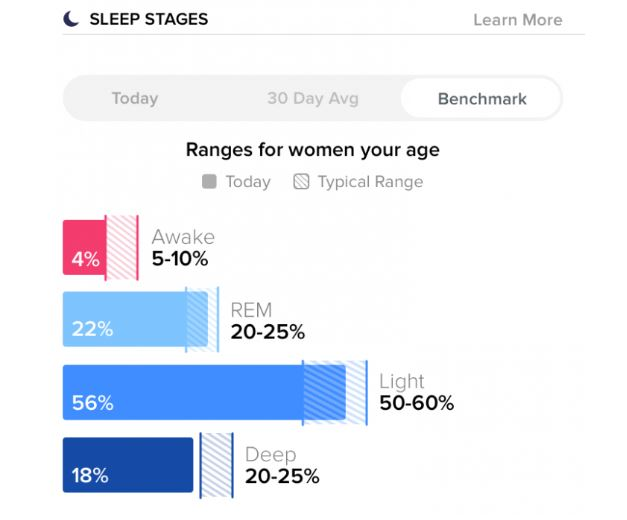
\includegraphics[width=.8\textwidth]{common-stages}
	\caption{Przyk�adowy podzia� stadi�w snu z opaski fitness.}\label{common-fitness-stages}
\end{figure}

U�atwieniem do przeprowadzania bada� nad snem, s� opaski fitness i smartwatche. Nie s� to urz�dzenia dok�adne jak EEG czy elektrokardiograf (EKG). Du�� zalet� jest jednak to, �e mog� rejestrowa� wyniki du�o cz�ciej ni� tradycyjne urz�dzenia i w d�u�szym okresie czasu. Nie wymagaj� przy tym od u�ytkownika �adnych umiej�tno�ci i nie utrudniaj� �ycia. Na rysunku (Rys~\ref{common-fitness-stages}) przedstawiono estymowany procentowy udzia� stadi�w i faz snu dla 30 letniej kobiety z por�wnaniem do innych kobiet w jej wieku. Dane te mog� pos�u�y� do analizy snu i przewidywania zachowa� poprzez stworzenie sztucznej sieci neuronowej. 

\chapter{Sie� neuronowa}
�Sie� neuronowa (sztuczna sie� neuronowa) � og�lna nazwa struktur matematycznych i ich programowych lub sprz�towych modeli, realizuj�cych obliczenia lub przetwarzanie sygna��w poprzez rz�dy element�w, zwanych sztucznymi neuronami, wykonuj�cych pewn� podstawow� operacj� na swoim wej�ciu. Oryginaln� inspiracj� takiej struktury by�a budowa naturalnych neuron�w, ��cz�cych je synaps, oraz uk�ad�w nerwowych, w szczeg�lno�ci m�zgu.

Czasem nazw� sztuczne sieci neuronowe okre�la si� interdyscyplinarn� dziedzin� wiedzy zajmuj�c� si� konstrukcj�, trenowaniem i badaniem mo�liwo�ci tego rodzaju sieci." ~\cite{wiki}

\begin{figure}[!htb]
	\centering
	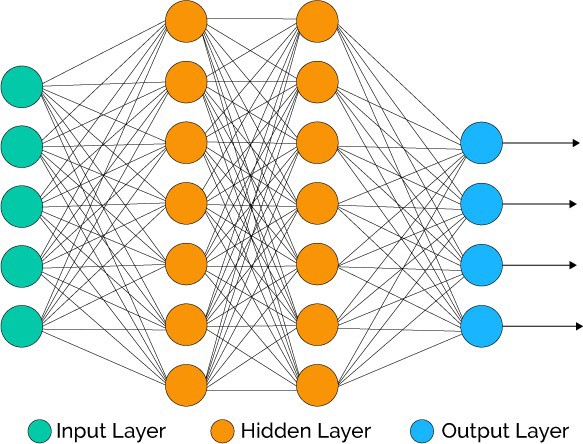
\includegraphics[width=.8\textwidth]{neural-network}
	\caption{Schemat wielowarstwowej sieci neuronowej.}\label{neural-network-img}
\end{figure}

Na rysunku (Rys.~\ref{neural-network-img}) przedstawiono schemat sztucznej sieci neuronowej. Elementami sk�adowymi s� wej�cia, ukryte pow�oki z wagami oraz wyj�cia sieci. Ilo�� pow�ok zale�y od konkretnych zastosowa� i nie jest jednoznaczna.

\section{Perceptron}
Najprostrz� sieci� neuronow� mo�e by� sztuczny neuron. Jest niedoskona�ym i uproszczonym modelem biologicznego neuronu, kt�ry jest zasadniczym elementem strukturalnym m�zgu. Por�wnanie neuronu oraz jego modelu przedstawiono na rysunku (Rys.~\ref{neuron-model-and-biology}).

\begin{figure}[!htb]
	\centering
	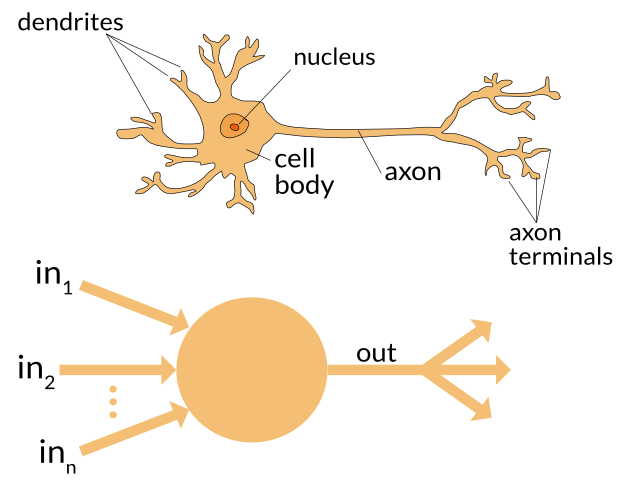
\includegraphics[width=.8\textwidth]{neuron-model-and-biology}
	\caption{Por�wnanie kom�rki nerwowej z jej modelem.}\label{neuron-model-and-biology}
\end{figure}

Rysunek (Rys.~\ref{perceptron-schema-img}) przedstawia schemat perceptronu. Jako $x$ oznaczono wej�cia sieci, $w$ - wagi neuron�w, $y$ to wyj�cie neuronu. S� to typowe oznaczenia stosowane w sieciach neuronowych. Od zwyk�ego sztucznego neuronu r�ni si� tym, �e zawiera funkcj� aktywacji, kt�ra zmienia warto�� wyj�cia, poprzez implementacj� wybranej funkcji. Do najcz�ciej u�ywanych funkcji aktywacji nale��:
\begin{itemize}
\item funkcja liniowa
\item funkcja progowa
\item funkcja sigmoidalna unipolarna
\item funkcja sigmoidalna bipolarna (tangens hiperboliczny)
\item funkcja Gaussa
\end{itemize}

\begin{figure}[!htb]
	\centering
	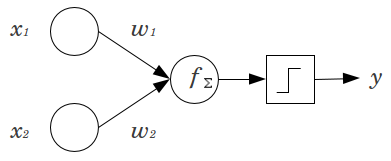
\includegraphics[width=.8\textwidth]{perceptron-schema}
	\caption{Schemat perceptronu.}\label{perceptron-schema-img}
\end{figure}

Wynikiem dzia�ania perceptronu jest warto�� z przedzia�u 0-1. W szczeg�lnych przepadkach - binaryzacji - warto�� wynosi dok�adnie 0 lub 1.
\section{Rekurencyjna sie� neuronowa}
Ludzki m�zg nie zaczyna �adnego swojego dzia�ania od zera. Ka�de nasze dzia�anie bazuje na do�wiadczeniach, kt�re s� sk�adowane w pami�ci. Podobnie dzia�a rekurencyjna sie� neuronowa (RNN - \textit{z ang. Recurent Neural Network}). Ka�da iteracja algorytmu uwzgl�dnia dane z poprzednich oblicze�, co przedstawia rysunek (Rys.~\ref{RNN-unrolled}. Dzi�ki temu sie� rozumie kontekst. Sieci te stosuje si� do rozpoznawania obraz�w, rozpoznawania mowy, t�umaczenia j�zyk�w. 

\begin{figure}[!htb]
	\centering
	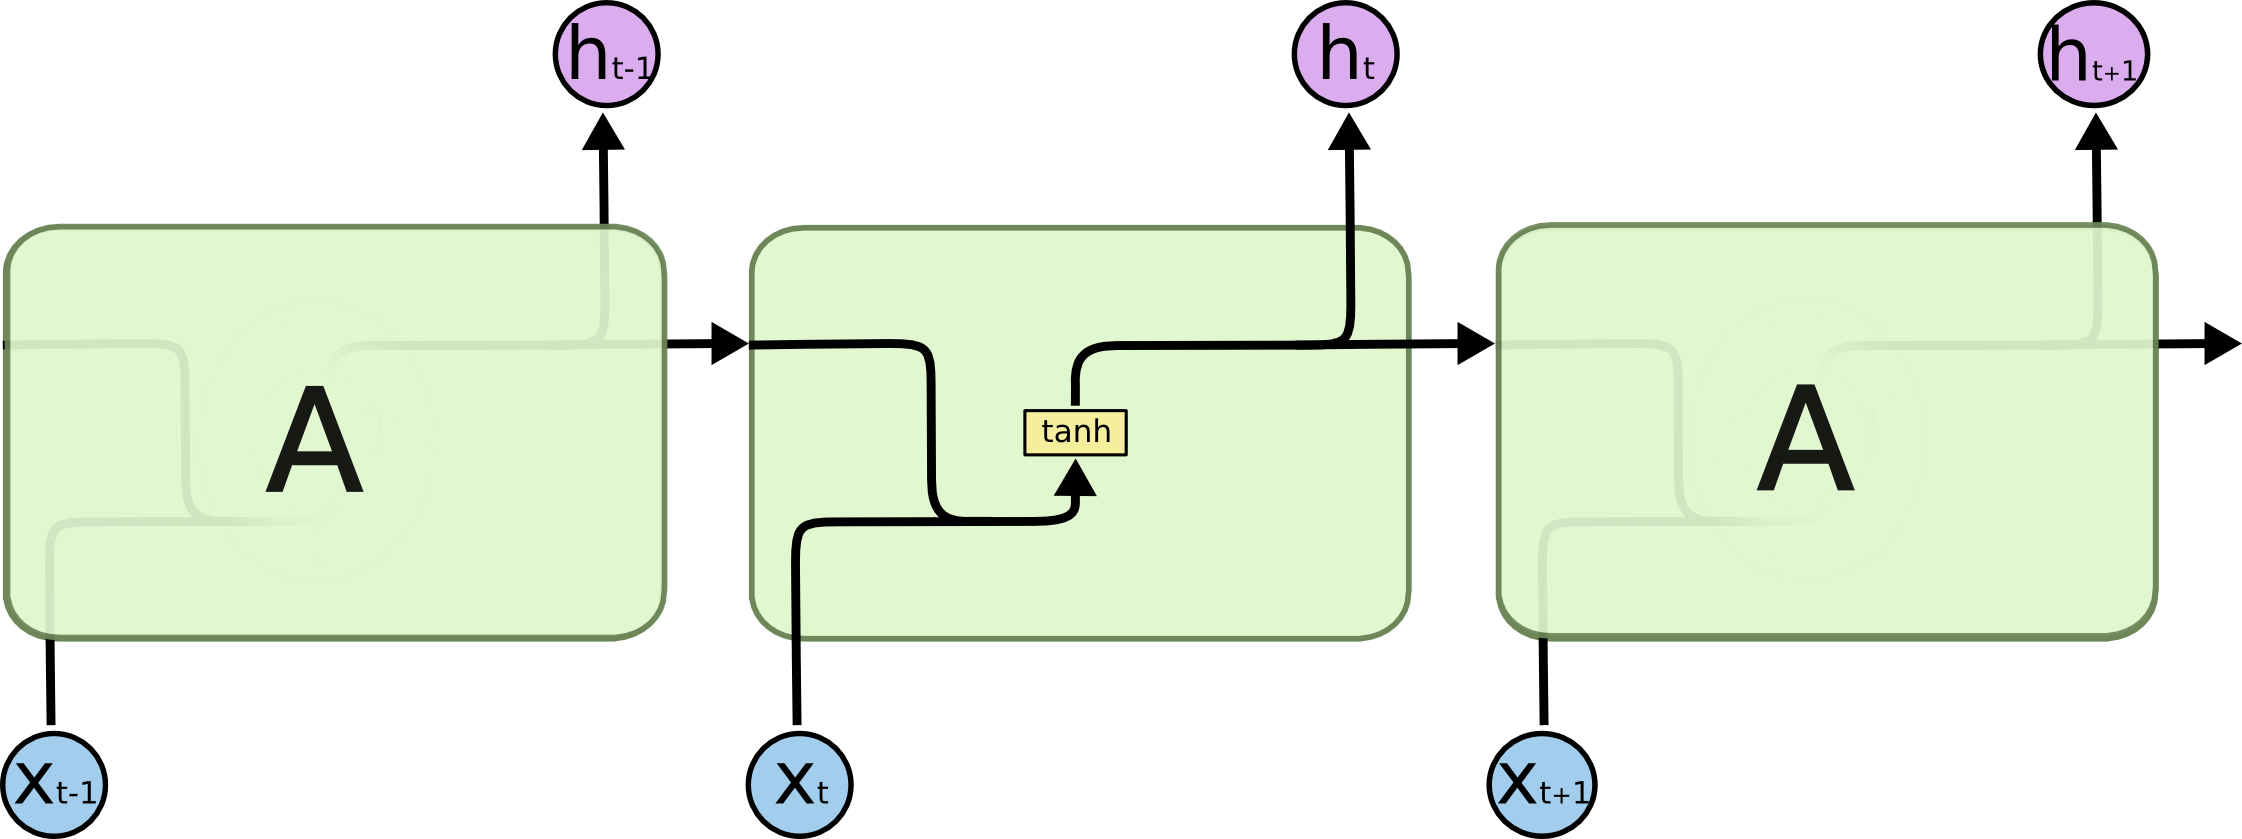
\includegraphics[width=1\textwidth]{common-RNN}
	\caption{Schemat rekurencyjnej sieci neuronowej.}\label{RNN-unrolled}
\end{figure}

\section{LSTM}
Long short-term memory (LSTM) jest specjalnym typem sieci rekurencyjnych. Technika ta nie posiada polskiego t�umaczenia. Pozwala na uczenie d�ugoterminowych zale�no�ci, kt�re s� ich typowym zastosowaniem. 

Model sieci LSTM przedstawia si� nast�puj�co: (Rys.~\ref{LSTM-RNN}).
\begin{figure}[!htb]
	\centering
	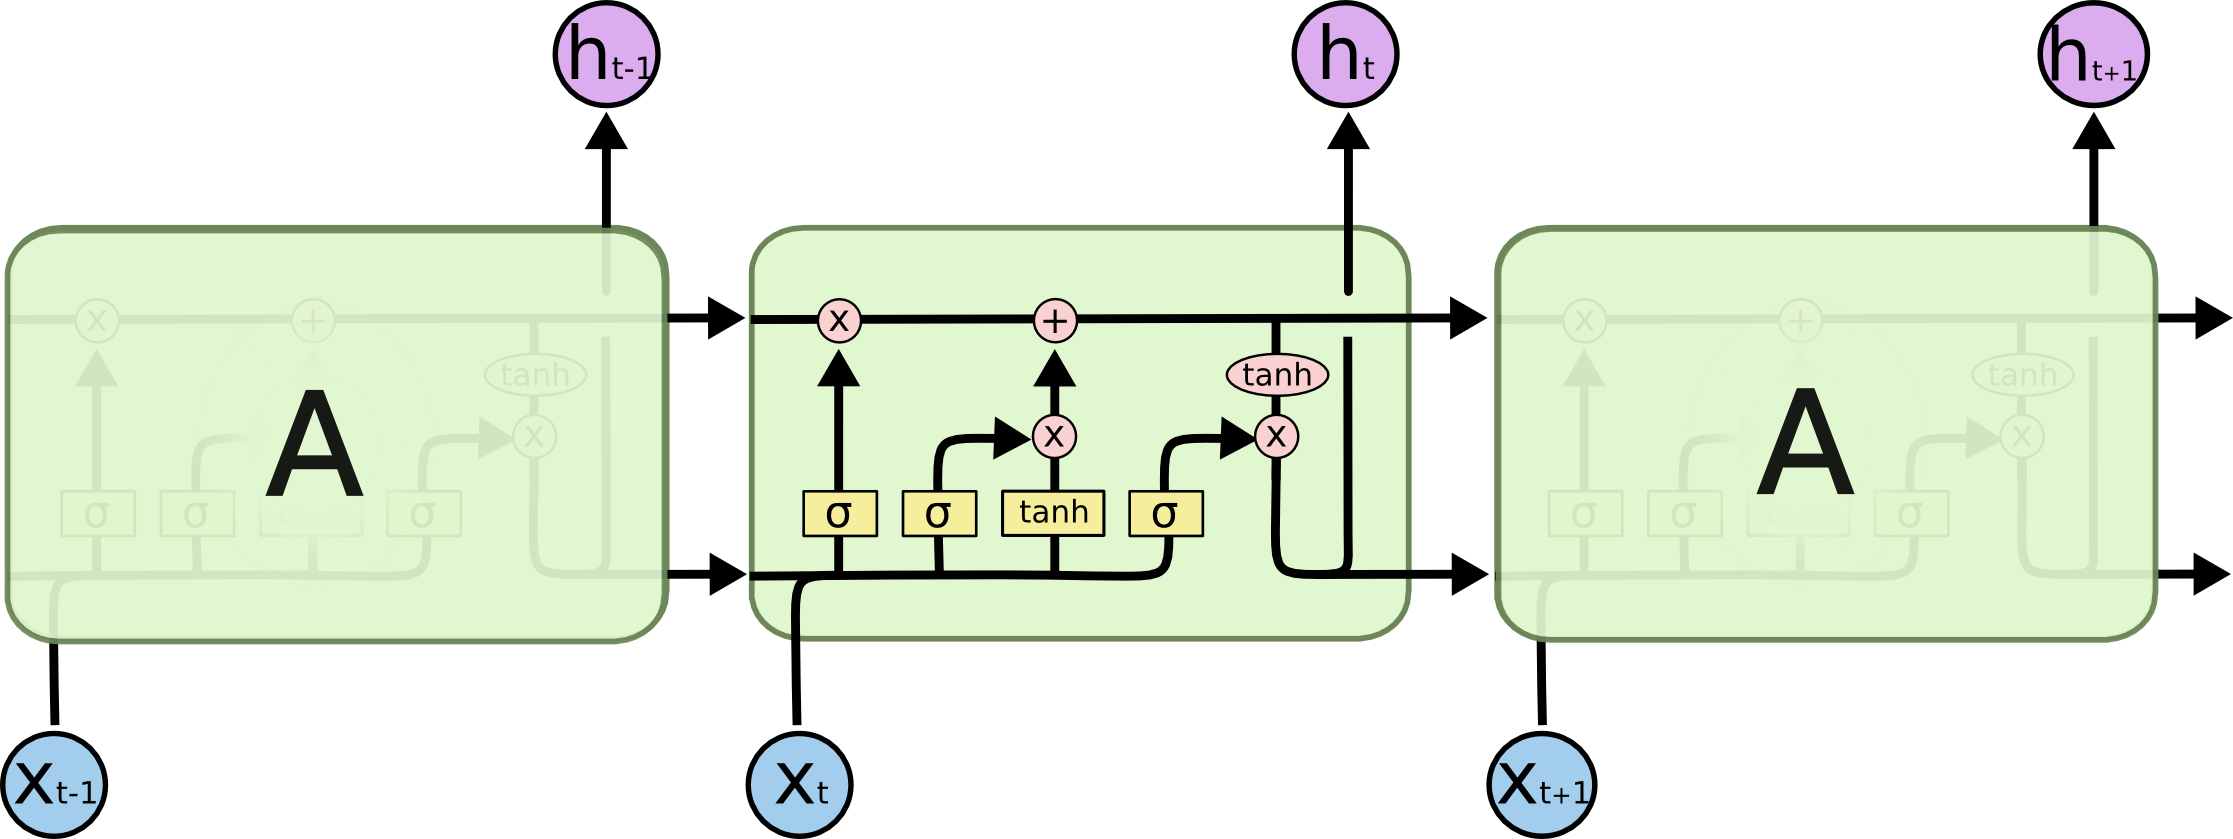
\includegraphics[width=1\textwidth]{LSTM-RNN}
	\caption{Schemat sieci LSTM.}\label{LSTM-RNN}
\end{figure}

LSTM u�ywa wewn�trz swojej pow�oki dw�ch funkcji aktywacji: sigmoidy unipolarnej oraz tangensa hiperbolicznego. Informacje ��cz� si� za pomoc� operacji mno�enia lub dodawania.

Schemat dzia�ania pojedynczego neuronu sk�ada si� z 4 krok�w(4 bram). Pierwszym z nich jest decyzja o tym czy przyj�t� informacj� nale�y zapomnie�. Decyzja jest podejmowana w oparciu o sigmoid� - je�li wynikiem jest 0 - nast�puje ca�kowite zamkni�cie bramy i zapomnienie informacji. 2 i 3 krokiem jest decyzja jakie warto�ci i z jakimi wagami nale�y zapami�ta� w pami�ci sieci. Wynik tej operacji w�druje do w�z�a sumacyjnego. Ostatnim krokiem jest obliczenie warto�ci wyj�cia sieci na podstawie poprzednich wynik�w oraz wszystkich wej�� sieci. 

Bardzo dobry, szczeg�owy artyku� o tym jak dzia�a RSTM mo�na przeczyta� pod linkiem \cite{lstm}. Rysunki o RNN zosta�y zaczerpni�te w�a�nie z tego �r�d�a. 
\chapter{Informacje techniczne}
Kod programu zosta� napisany w j�zyku \textit{Python} w wersji 3.6. Jako �rodowiska programistycznego u�yto \textit{Spyder}. Korzystano z bibliotek: do sieci neuronowych \textit{Keras}, kt�ry jako silnika u�ywa biblioteki \textit{Tensorflow}, do oblicze� matematycznych: \textit{sklearn}, do tworzenia wykres�w: \textit{matplotlib}. Dane pochodz�ce od badanego by�y przechowywane w pliku CSV.
\chapter{Dane wej�ciowe}
\section{Zbieranie danych}
Dane do sieci neuronowej zosta�y zebrane za pomoc� opaski fitness \textit{Xiaomi Mi Band 2} oraz telefonu z systemem \textit{Android} z zainstalowan� aplikacj� \textit{Mi Fit}. Opaska umo�liwia monitorowanie snu. Dane s� zbierane poprzez akcelerometr, kt�ry s�u�y do pomiaru przy�piesze� liniowych i k�towych. Aplikacja analizuje te dane i na ich podstawie estymuje czas snu lekkiego i g��bokiego, wed�ug ruchowej aktywno�ci w nocy. Przyk�adowe interpolowane ju� dane z jednej nocy przedstawiono na rysunku (Rys.~\ref{sleep-acc-data}). 
\begin{figure}[!htb]
	\centering
	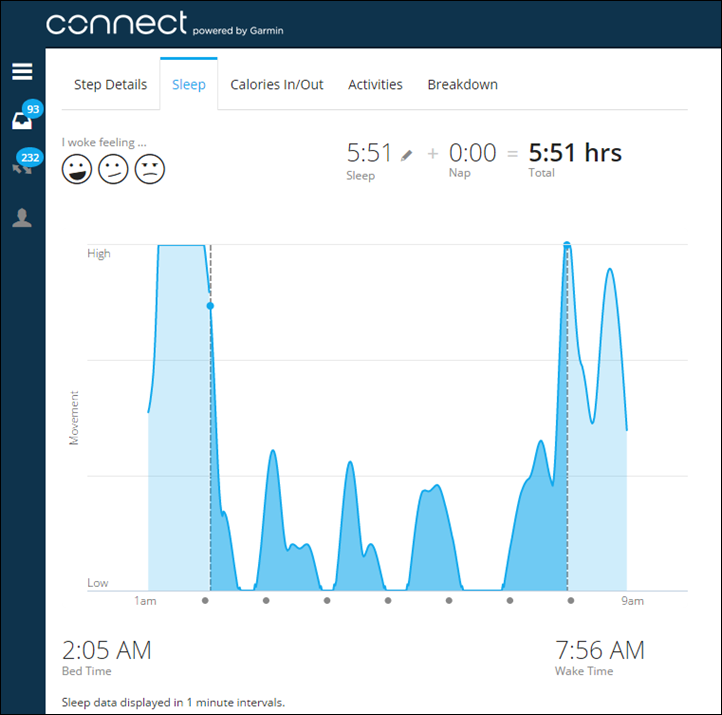
\includegraphics[width=0.8\textwidth]{sleep-acc-data}
	\caption{Przyk�adowe dane snu z opaski fitness.}\label{sleep-acc-data}
\end{figure}

Za pomoc� tej metody zebrano dane snu z 200 dni, od jednej osoby w wieku 16 lat.
\section{Przygotowywanie danych}
Dane do sieci musz� zosta� znormalizowane. Do tego celu u�yto gotowej funkcji \textit{MinMaxScaler} z biblioteki \textit{sklearn.preprocessing}. Funkcja korzysta ze wzoru:
\[x_{odch} = \frac{ x - min(X)}{max(X) - min(X)}\]
\[x_{norm} = x_{odch} * (max - min) + min\]
Przy czym: 
\begin{itemize}
\item x to dana wej�ciowa
\item X to zbi�r danych typu x
\item min(X) to minumum ca�ego zbioru
\item min to najmniejsza liczba po normalizacji
\end{itemize}
Normalizacj� przeprowadzono do warto�ci z przedzia�u 0-1. 

Niekt�re z danych by�y formatu data-czas. W tym wypadku obliczono ilo�� czasu od p�nocy w minutach. Dodatkowo dostarczano dane o dniu tygodnia - dni zosta�y zamienione na liczby ca�kowite z przedzia�u 0-6. Wszystkie dane wej�ciowe zosta�y znormalizowane. 

Jako, �e testowany typ sieci uczy si� z nadzorem, zbi�r danych podzielono na zbi�r ucz�cy oraz testowy w proporcji 0.85/0.15. 

LSTM z ka�d� iteracj� przetwarza nie tylko jedno wej�cie, ale tak�e wej�cia z poprzednich iteracji. Dlatego jako wej�cia nale�a�o przygotowa� tablic� sk�adaj�c� si� z 3 wymiar�w: wej�cia sieci, codzienne dane oraz wektory z danymi z poprzednich \textit{x} iteracji, gdzie \textit{x} oznacza liczb� poprzednich krok�w, kt�re bierzemy pod uwag� w sieci. 

\chapter{Model sieci}
\section{Wej�cia sieci}
Jako wej�cia sieci ustalono:
\begin{itemize}
\item czas za�ni�cia
\item czas obudzenia 
\item dzie� tygodnia
\end{itemize}
\section{Wyj�cia sieci}
Wyj�ciem sieci jest jako�� snu definiowana jako:
\[\text{Jako�� snu} = \frac{\text{Ilo�� snu g��bokiego}}{\text{Ca�kowita ilo�� snu}}\]
\section{Pow�oki}
W trakcie bada� wyznaczono do�wiadczalnie sie� sk�adaj�c� si� z 4 pow�ok z 50 neuronami na ka�dej pow�oce. 

\begin{figure}[!htb]
	\centering
	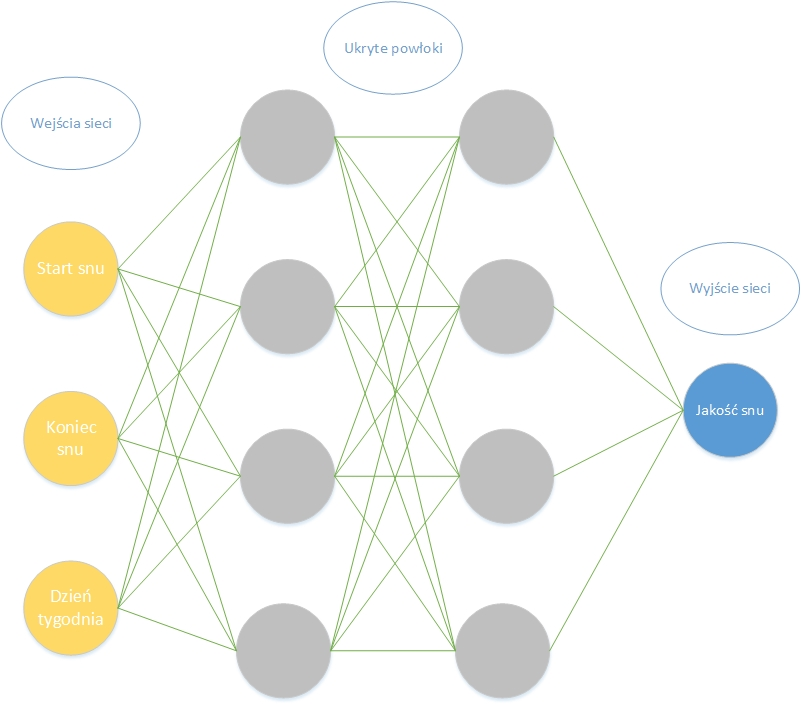
\includegraphics[width=1\textwidth]{lstm_schema}
	\caption{Zaprojektowana sie� neuronowa.}\label{lstm-schema}
\end{figure}

Rysunek (Rys.~\ref{lstm-schema}) przedstawia model zaprojektowanej sieci neuronowej. 
\chapter{Wyniki}
Podczas bada� sieci starano dostosowa� parametry pod k�tem najmniejszego b��du �redniokwadratowego oraz najlepszego wizualnego dopasowania funkcji (uwzgl�dniaj�c przy tym zmiany wolnofalowe).

Do�wiadczalnie zosta�y wyznaczone nast�puj�ce parametry:
\begin{itemize}
\item ilo�� epok: 1000
\item dropout: 20\%
\item mini-batch: 8
\item poprzednie kroki: 32
\end{itemize}

Na rysunkach (Rys.~\ref{TS32} i ~\ref{TS32E})  przedstawiono najlepsze odwzorowanie zbioru testowego. Zbi�r posiada� 30 danych wej�ciowych - czyli 30 dni. 
\begin{figure}[!htb]
	\centering
	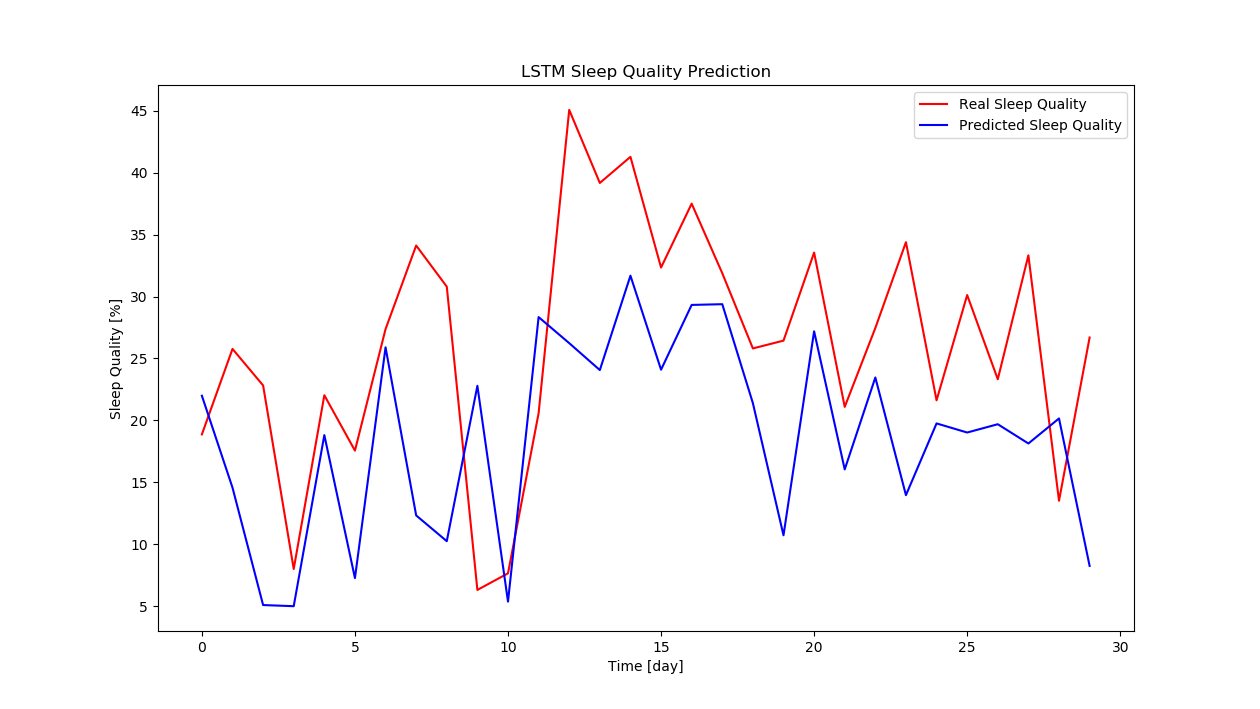
\includegraphics[width=1\textwidth]{TS32}
	\caption{Predykcja jako�ci snu.}\label{TS32}
\end{figure}
\begin{figure}[!htb]
	\centering
	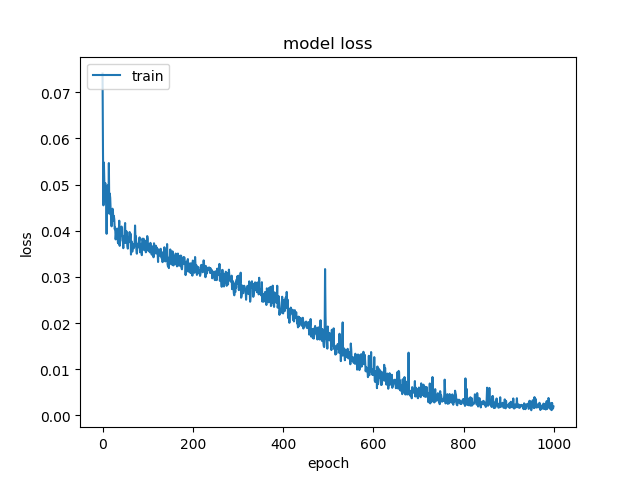
\includegraphics[width=1\textwidth]{TS32E}
	\caption{Funkcja b��du �redniokwadratowego od epok sieci.}\label{TS32E}
\end{figure}

\section{Trudno�ci rozwi�zania}
Wyznaczenie prawid�owych wynik�w przez sie� by�o bardzo trudne, poniewa� w ci�gu ostatniego miesi�ca, osoba badana odnotowa�a znaczny wzrost jako�ci snu. Przewidzenie takiego zachowania jest prawie niemo�liwe dla sieci. Rysunek (Rys.~\ref{dataset}) przedstawia jako�� snu badanego w ci�gu ca�ego okresu akwizycji danych. Linia pionowa oddziela dane ucz�ce sie� od danych testowych. Mo�liwym ulepszeniem algorytmu by�oby rozproszenie danych testowych w�r�d wszystkich danych. Jest to skomplikowany krok, poniewa� ka�da dana potrzebuje dane z poprzednich iteracji, jednak mo�liwe do osi�gni�cia na wi�kszym zbiorze danych. 

\begin{figure}[!htb]
	\centering
	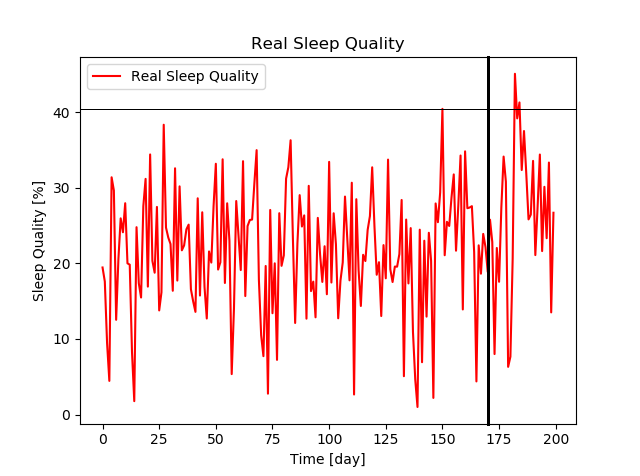
\includegraphics[width=0.8\textwidth]{dataset}
	\caption{Jako�� snu badanego.}\label{dataset}
\end{figure}

\section{Dodatek}
Na pocz�tku pracy z projektem rozwa�ano zastosowanie prostej sieci wielowarstwowej (MLP z \textit{ang. Multilayer perceptron}). Jednak sie� okaza�a si� wychwytywa� tylko jedno rozwi�zanie funkcji, szybko si� przeucza�a - wyj�cie sieci nie zale�a�o ju� od wej��, funkcja by�a okresowa.  Mo�na zobaczy� to na rysunku (Rys. ~\ref{MLP}). W tamtym algorytmie testowano 2 wyj�cia sieci - czas obudzenia i jako�� snu.

\begin{figure}[!htb]
	\centering
	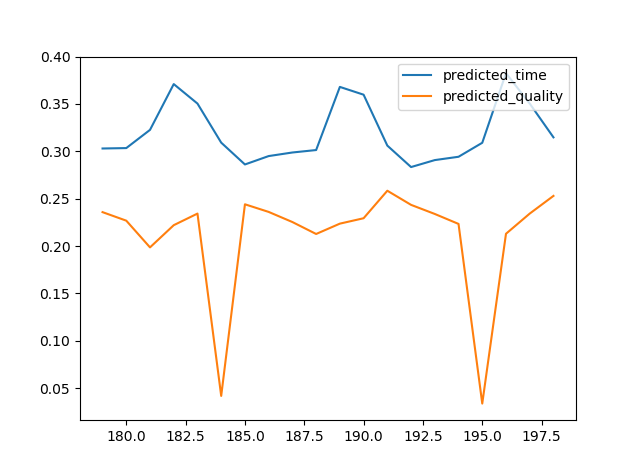
\includegraphics[width=0.8\textwidth]{MLP}
	\caption{Dodatek: MLP do przewidywania snu.}\label{MLP}
\end{figure}

\chapter{Wnioski}
\begin{itemize}
\item Sieci neuronowe s� interesuj�cym do dalszych bada� narz�dziem do badania i przewidywania biologicznych zale�no�ci, na przyk�ad zagadnienia snu. 
\item Nie uda�o si� wyznaczy� dok�adnej optymalnej ilo�ci snu dla badanej osoby. Utworzono jednak sie�, kt�ra z zadowalaj�c� dok�adno�ci� rozumie korelacj� mi�dzy godzinami snu a jego jako�ci�. 
\item Czas, jako dana u�ywana w sieci, nie jest intuicyjnie rozumiana przez sie�. Sieci LSTM naturalnie powinny radzi� sobie z tego typu informacjami, jednak zaimplementowanie ich do algorytmu, wi��e si� z przyj�ciem pewnej abstakcji. Na skonstruowanie wej�� czasowych nie ma jednego sposobu. Od przetworzenia tych danych zale�y pomy�lno�� wynik�w. 
\item Wybrana ilo�� poprzednich krok�w (32) jest bardzo du�a. Mo�e to �wiadczy� o tym, �e nasz sen zale�y od wielu poprzednich dni.
\item Dob�r parametr�w wp�ywa na wyniki. Cz�sto lepiej doda� wi�cej pow�ok i iteracji, trac�c troch� czasu, ale otrzymuj�c nie gorsze wyniki. Nale�y jednak pami�ta� o zjawisku przeuczenia sieci.
\item Post�p uczenia sieci oraz jej prawid�owo��, najlepiej ocenia� analizuj�c b��d �redniokwadratowy - ten sam, kt�ry sie� u�ywa do dopasowywania wag neuron�w. Cennym przy analizie i doborze parametr�w jest wyrysowanie funkcji b��du �redniokwadratowego od epok algorytmu. Bardzo �atwo w ten spos�b dobra� odpowiedni� ilo�� epok.
\item Aby wnioski by�y w pe�ni poprawne, zamodelowana sie� neuronowa powinna by� przebadana na wi�kszej liczbie badanych i wi�kszej liczbie pr�bek.
\item Projekt ten jest �atwo rozszerzy� o kolejne dane i wej�cia sieci. 
\item Por�wnywano u�ywanie biblioteki Keras z silnikiem Tensorflow do tradycyjnego Tensorflow. Biblioteka Keras znacz�co u�atwia prac� z sieciami neuronowymi. Pozwala zaimplementowa� dowoln� sie� w kilku krokach. Na tym poziomie tworzenia i badania, jest to najlepszy wyb�r. 
\item Podczas realizowania projektu uczy�em si� podstaw Pythona oraz jego bibliotek. Nie stanowi�o to jednak wi�kszego problemu w pracy. Ca�e �rodowiko jest intuicyjne, a biblioteki pozwalaj� na implementacj� kompletnych, gotowych funkcji matematycznych, takich jak obliczanie b��du �redniokwadratowego, normalizacje czy transponowanie macierzy. 
\end{itemize}

\chapter{Dalszy rozw�j projektu}
W przysz�o�ci planowane jest zebranie wi�kszej ilo�ci danych i dalsze testowanie sieci. Mo�liwe jest tak�e stworzenie algorytmu, kt�ry na podstawie utworzonej w tym projekcie sieci, b�dzie przewidywa�, o kt�rej nale�y po�o�y� si� spa�, �eby najlepiej si� wyspa�. Na t� chwil� jednak, sie� nie jest wystarczaj�co przetestowana i wiarygodna, aby opiera� na niej inne algorytmy i badania.

Planowane jest tak�e rozszerzenie sieci o nowe wej�cia. Na pewno znalaz�yby si� tam dane o aktywno�ci fizycznej w ci�gu dnia, kt�re tak�e mo�na sczyta� z opaski fitness. Dodatkowo mo�liwe jest zebranie informacji o drzemkach w ci�gu dnia oraz wypitych kawach.

\appendix  % <--- zaczynaj� si� dodatki; jak nazywa si� rozdzia� -> szuka� appendixname powy�ej
\chapter{Dodatek A}
W dodatku umieszczamy opis ewentualnych znanych algorytm�w, z kt�rych korzystamy proponuj�c w�asn� metodologi�, opisan� w rozdziale~\ref{Chapter_Metodologia}. Wykaz pozycji literaturowych tworzymy w oddzielnym pliku \texttt{Praca.bib}. Chc�c si� odwo�a� w tek�cie do wybranej pozycji bibliograficznej korzystamy z komendy \texttt{cite}. Efekt jej u�ycia dla kilku pozycji jednocze�nie to~\cite{Tadeusiewicz,Malina,Nieniewski_Morfologia}.

%%%%%%%%%%%%%%%%%%%%%%%%%%%%%%%%%%%%%%%%%%%%%%%%%%%%%%%%%%%%%%%%%%%%%%%%%%%%%%%%%%%%%%%%%%%%%%%%%%%%%%%%%%%%%%%%%%%%%%%%%%%%%%%%%%%%%%%%%%%%%%%%%%%%%%%%%%%%%%%%%%%%%%%
\chapter{Dodatek B}
Podstawowe kwestie techniczne dotycz�ce wzor�w, rysunk�w, tabel poni�ej.

Wzory tworzymy w �rodowisku \texttt{equation}. Chc�c odwo�a� si� do wybranego wzoru gdzie� w tek�cie nale�y nada� mu stosown�, niepowtarzaln� i jednoznaczn� etykiet�, po ty by m�c np. napisa� zdanie: ze wzoru~\ref{Wzor_Dodawanie} wynika \ldots
\begin{equation}\label{Wzor_Dodawanie}
	c = a + b
\end{equation}

Wzory z�o�one, charakteryzuj�ce si� przypisaniem warto�ci zmiennej w pewnych okoliczno�ciach tworzymy przy u�yciu otoczenia \texttt{eqnarray}. Odwo�anie do wzoru jak wcze�niej. 
\begin{eqnarray}\label{equ_progowanie}
    BW & = & \left \{
    \begin{array}{ll}
      1, & I(x,y) \geq T \\
      0, & I(x,y) < T\\
    \end{array}
    \right.,
\end{eqnarray}

% \subsection{Usuwanie numeracji przy r�wnaniach}

Numeracj� r�wna� mo�na tymczasowo (w~danej linijce) wy��czy� poprzez u�ycie $\backslash{}nonumber$
\begin{eqnarray}
	a_i = a_{i-1}+a_{i-2}\nonumber \\ % w tej linijce nie ma numeru
              +a_{i-3}
\end{eqnarray}


\section{Wstawianie rysunk�w}
Rysunki umieszczamy w otoczeniu \texttt{figure}, centruj�c je w poziomie komend� \texttt{centering}. Rozmiary rysunku ustalamy w komendzie \texttt{includegraphics} dobieraj�c wielko�� wzgl�dem rozmiaru strony lub bezwzgl�dnie np. w cm. Ponadto najpierw zapowiadamy pojawienie si� rysunku w tek�cie (czyli np. Na rysunku (Rys~\ref{Rysunek_LogoIB}) pracy, a dopiero p�niej wstawiamy sam rysunek. Dodatkowo sterowa� mo�emy umiejscowieniem rysunku na stronie dzi�ki parametrom \texttt{[!htb]} okre�laj�cym miejsce. Odpowiednio s� to: \texttt{here}, \texttt{top}, \texttt{bottom}. 
\begin{figure}[!htb]
	\centering
	
\includegraphics[width=.35\textwidth]{logoRIB}
	\caption{Logo Wydzia�u In�ynierii Biomedycznej.}\label{Rysunek_LogoIB}
\end{figure}

Do��czaj�c rysunki nie trzeba podawa� rozszerzenia (wr�cz jest to odradzane). Je�li rysunki znajduj� si� w~katalogu \emph{rysunki}, nie trzeba r�wnie� podawa� �cie�ki do nich.

\section{Wstawianie tabelek}
Analogicznie post�pujemy z tabelkami, z t� r�nic� �e tworzymy j� w otoczeniu \texttt{table}. W nim natomiast sam� tabel� definiujemy albo w �rodowisku \texttt{tabular}, albo \texttt{tabularx}. Podobnie z odwo�aniami w tek�cie: najpierw odwo�anie w Tab.~\ref{Tabelka_Tabela}, a dopiero p�niej sama tabela.
\begin{table}[!htb]
	\centering
	\topcaption{Opis nad tabelk�.}\label{Tabelka_Tabela}
	\begin{tabular}{|c|c|c|c|} \hline \hline 
		Kolumna 1 & Kolumna 2 & Kolumna 3 & Kolumna 4 \\ \hline
		Wiersz 1 & & & \\ \hline
		Wiersz 2 & & & \\ \hline
		Wiersz 3 & & & \\ \hline
		& & & \\ \hline
		& & & \\ \hline
	\end{tabular}
\end{table}

%%%%%%%%%%%%%%%%%%%%%%%%%%%%%%%%%%%%%%%%%%%%%%%%%%%%%%%%%%%%%%%%%%%%%%%%%%%%%%%%%%%%%%%%%%%%%%%%%%%%%%%%%%%%%%%%%%%%%%%%%%%%%%%%%%%%%%%%%%%%%%%%%%%%%%%%%%%%%%%%%%%%%%%
\chapter{Kwestie edytorskie}
Zbi�r zasad pomocnych przy redagowaniu tekstu pracy wystarczaj�co szczeg�owo przedstawia ksi��ka~\cite{Chwalowski}.

Uwaga! Pisz�c prac� nale�y zwr�ci� uwag� na nast�puj�ce kwestie:
\begin{enumerate}
	\item Prace piszemy w formie bezosobowej.
	\item Unikamy okre�le� potocznych, spolszcze� funkcjonuj�cych codziennej mowie itp.
	\item Pos�uguj�c si� znanymi nam (a nie czytelnikowi) has�ami (r�wnie� skr�tami, akronimami) najpierw je definiujemy i~t�umaczymy, a~dopiero p�niej traktujemy za znane.
	\item Podpisy pod rysunkami lub nad tabelami traktujemy jak zdania, a wi�c powinny stanowi� sp�jn� ca�o�� oraz powinny zosta� zako�czone kropk�.
	\item Podobnie wypunktowania (po dwukropku kolejne punkty pisane ma�ymi literami, oddzielane przecinkami, ostatni zako�czony kropk� o ile ko�czy zdanie).
	\item Do ka�dego rysunku, tabeli, pozycji bibliograficznej musi istnie� odwo�anie w tek�cie pracy, przy czym do pierwszych dw�ch musi si� ono pojawi� zanim umie�cimy rysunek/tabel�.
\end{enumerate}


\clearpage \addcontentsline{toc}{chapter}{\bibname}
\bibliography{Praca}


\end{document}
